\subsection{normalisation}
It is recommended that the tumour volume data get normalised before the visual and representative analysis is carried out \autocite{Heitjan:1993uw,Demidenko:2010gn}.
Tumour volume distribution is usually skewed and influenced by the outliers, in particular if sample is small, leading to imprecise outcomes and power reductions.
Making the distribution more Gaussian looking helps in reducing this bias and leads to a better power and more statistically significant treatment effects.
The most popular normalising technique is a log-transformation.
It is stabilising the tumour volume variance and given its monotonic property it does not affect the data content.
Therefore it is recommended but may require results to be back-transformed once interpreted.
\Cref{raw_trajectories_log_reduced_follow-up} presents the log$_{10}$-transformed original data (see \cref{raw_trajectories}) over the selected follow-up sub-period.
Given that the log function is not defined for zero volumes they needs to be imputed as zeros on a log-scale.
The follow-up period was reduced to the most relevant part.
It starts on day 6 when the animals get randomised among the treatment groups, and ends-up on day 27 where there are at least two alive animals per treatment line.
The log-transformed trajectories present an exponential growth pattern.


\begin{figure}
	\centering
	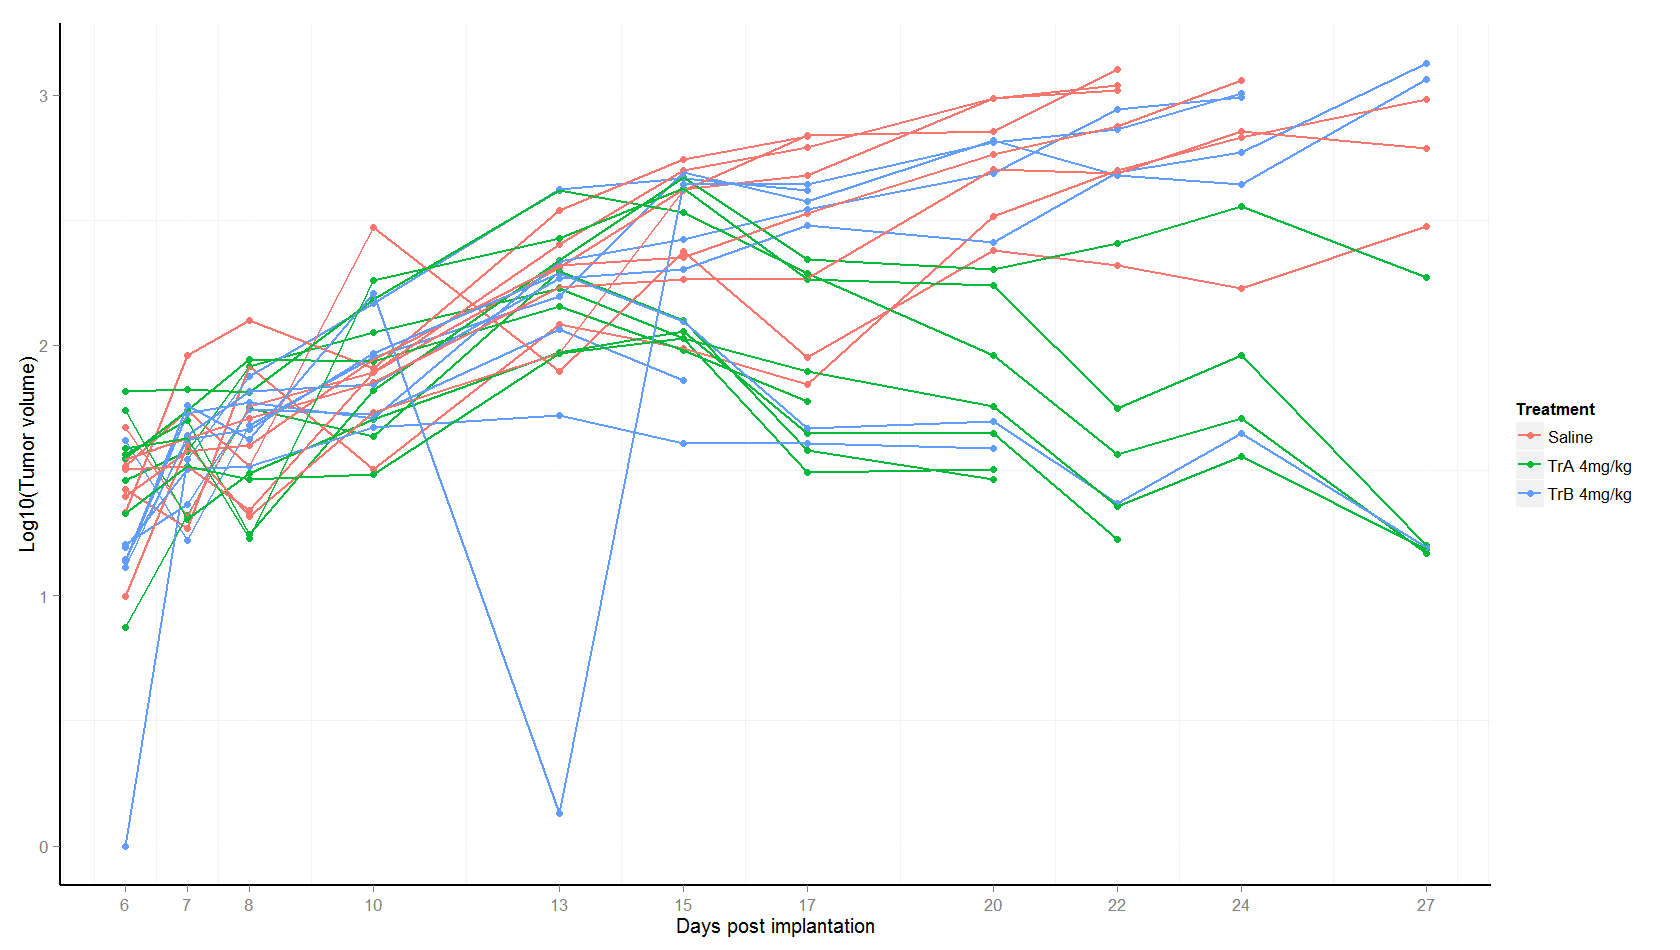
\includegraphics[width=\textwidth]{xenograph/figures/raw_trajectories_log_reduced_follow-up.png}
	\caption{Empirical tumour volume (mm$^3$) trajectories after log$_{10}$-transformation.}
	\label{raw_trajectories_log_reduced_follow-up}
\end{figure}
